%; whizzy paragraph -pdf xpdf -latex ./whizzypdfptex.sh
%; whizzy-paragraph "^\\\\begin{frame}"
% latex beamer presentation.
% platex, latex-beamer $B$G%3%s%Q%$%k$9$k$3$H$rA[Dj!#(B 

%     Tokyo Debian Meeting resources
%     Copyright (C) 2009 Junichi Uekawa
%     Copyright (C) 2010 Nobuhiro Iwamatsu

%     This program is free software; you can redistribute it and/or modify
%     it under the terms of the GNU General Public License as published by
%     the Free Software Foundation; either version 2 of the License, or
%     (at your option) any later version.

%     This program is distributed in the hope that it will be useful,
%     but WITHOUT ANY WARRANTY; without even the implied warranty of
%     MERCHANTABILITY or FITNESS FOR A PARTICULAR PURPOSE.  See the
%     GNU General Public License for more details.

%     You should have received a copy of the GNU General Public License
%     along with this program; if not, write to the Free Software
%     Foundation, Inc., 51 Franklin St, Fifth Floor, Boston, MA  02110-1301 USA

\documentclass[cjk,dvipdfm,12pt]{beamer}
\usetheme{Tokyo}
\usepackage{monthlypresentation}
%  preview (shell-command (concat "evince " (replace-regexp-in-string "tex$" "pdf"(buffer-file-name)) "&"))
%  presentation (shell-command (concat "xpdf -fullscreen " (replace-regexp-in-string "tex$" "pdf"(buffer-file-name)) "&"))
%  presentation (shell-command (concat "evince " (replace-regexp-in-string "tex$" "pdf"(buffer-file-name)) "&"))

%http://www.naney.org/diki/dk/hyperref.html
%$BF|K\8l(BEUC$B7O4D6-$N;~(B
\AtBeginDvi{\special{pdf:tounicode EUC-UCS2}}
%$B%7%U%H(BJIS$B7O4D6-$N;~(B
%\AtBeginDvi{\special{pdf:tounicode 90ms-RKSJ-UCS2}}

\title{$BEl5~%(%j%"(B Debian $BJY6/2q(B}
\subtitle{$B;qNA(B}
\author{$B>e@n=c0l(B dancer@debian.org\\IRC nick: dancerj}
\date{2010$BG/(B03$B7n(B20$BF|(B}
\logo{
\includegraphics[width=8cm]{image200607/openlogo-light.eps}}

\begin{document}

\frame{\titlepage{}}

\emtext{$B@_1D=`Hw$K$46(NO$/$@$5$$(B}

\begin{frame}
 \frametitle{$BJY6/2q$NO"Mm;v9`(B}
\begin{minipage}[t]{0.45\hsize}
  \begin{itemize}
   \item $BCm0U;v9`(B
	 \begin{itemize}
	  \item $B0{?)(B?
	 \end{itemize}
  \end{itemize}
\end{minipage} 
\begin{minipage}[t]{0.45\hsize}
 \begin{itemize}
  \item $B%K%e!<%i%k%M%C%H%o!<%/$G2hA|$rJ,N`$7$F$_$?(B
  \item weka
  \item libfftw
  \item man-db $B?<DI$$(B
  \item dpkg v3 quilt
 \end{itemize}
\end{minipage}
\end{frame}

\begin{frame}{Hack Cafe}
 $B:G6a%O%C%/%+%U%'$7$F$^$9$+(B?
 \url{http://twitter.com/debian_hackcafe}\\
\end{frame}

\emtext{$B;vA02]Bj(B}

\begin{frame}{$B;vA02]Bj(B}
\begin{enumerate}
 \item $B9%$-$JF|K\8l(BMan$B%Z!<%8(B
 \item $B%K%e!<%i%k%M%C%H%o!<%/$G2r7h$G$-$kLdBj(B
\end{enumerate}
\end{frame}

{\footnotesize

% this is a prework file.

}

% ------------------------------------------------------------------------------
\emtext{$B%K%e!<%i%k%M%C%H%o!<%/$G2hA|$rJ,N`$7$F$_$?(B}
% ------------------------------------------------------------------------------

% ------------------------------------------------------------------------------
\emtext{Debian$B$G(Bweka$B$r;H$C$F$_$k(B}
% ------------------------------------------------------------------------------

% ------------------------------------------------------------------------------
\emtext{Debian$B$G(Blibfftw$B$r;H$C$F$_$k(B}
% ------------------------------------------------------------------------------

\begin{frame}{$B$O$8$a$K(B}
$B2;@<%G!<%?$N2r@O!"$H$j$"$($:$^$:(B FFT $B$r$+$1$k!#(B

Debian$B$G(BFFT$B=hM}$r$9$k$?$a$N%9%F%C%W$H$7$F!"2;@<%G!<%?$N%m!<%I$H(BFFT$B=hM}$,(B
$B$"$k!#(B
$B%3!<%I$r=q$$$F$_$k$N$K!"(BDebian$B%Q%C%1!<%8$r3hMQ$9$k(B

\begin{itemize}
 \item $B2;@<%G!<%?$N:n@.(B: $BE,Ev$J%D!<%k$r;H$&(B
 \item $B2;@<%G!<%?$N%m!<%I(B: sndfile 
 \item FFT$B=hM}(B: libfftw
 \item $B7k2L$N=hM}(B: R
\end{itemize}
\end{frame}

\begin{frame}[containsverbatim]{$B:`NA$H$J$k2;@<%G!<%?$r=`Hw(B}

aeolus $B$r(B vkeybd $B$G(B midi $B@)8f$7$D$D!"(Becasound $B$G(B jack $B7PM3$G2;@<$rO?2;!#(B
sweep $B$G8e$GE,@Z$J%5%$%:$K@Z$j=P$9!#(B

\begin{commandline}
$ qjackctl &
$ aeolus &
$ vkeybd &
$ ecasound -i jack -o test.wav
ctrl-C $B$GCfCG(B
$ sweep test.wav # $BE,Ev$KJT=8(B
$ file ra-mono.wav  # $B@Z$j=P$7$?7k2L$r3NG'(B
ra-mono.wav: RIFF (little-endian) data, WAVE audio, 
Microsoft PCM, 16 bit, mono 44100 Hz
\end{commandline}
 
\end{frame}

\begin{frame}[containsverbatim]{$BI,MW$J%Q%C%1!<%8$r%$%s%9%H!<%k(B}
 
\begin{commandline}
$ apt-get install libfftw3-dev libsndfile1-dev
\end{commandline}

\end{frame}

\begin{frame}[containsverbatim]{$B%3!<%I$r=q$$$F$_$?(B1: sndfile}

sndfile $B$NDs6!$9$k(BAPI$B$r;H$$!"(B double $B$NG[Ns$K2;@<%G!<%?(B(wav $B%U%!%$%k(B)$B$r(B
$BFI$_9~$`!#(B

\begin{commandline}
  SF_INFO sfinfo = {0, 0, 0, 0, 0, 0};
  SNDFILE* s = sf_open(filename, SFM_READ, &sfinfo);
  double* data = malloc(sizeof(double) * size);
  sf_readf_double(s, data, size / sfinfo.channels);
  study_sound(data, size / sfinfo.channels);
  sf_close(s);
\end{commandline} 
\end{frame}

\begin{frame}[containsverbatim]{$B%3!<%I$r=q$$$F$_$?(B2: FFT}

FFTW $B$NDs6!$9$k(BAPI$B$r;H$$!"(Bdouble $B$NG[Ns$r(BFFT$B=hM}!"7k2L$rJ#AG?t$NG[Ns$K$$(B
$B$l$k!#(B

\begin{commandline}
  fftw_complex* spectrum;
  fftw_plan p;
  spectrum = (fftw_complex*) fftw_malloc(
    sizeof(fftw_complex) * (size / 2 + 1));
  p = fftw_plan_dft_r2c_1d(size, data, spectrum, FFTW_ESTIMATE);
  fftw_execute(p);
\end{commandline} 
\end{frame}

\begin{frame}[containsverbatim]{R$B$G%0%i%U$K$7$F$_$?(B}

$B7k2L$rE,Ev$K(Bcsv$B$G=PNO$7$F!"%0%i%U$K$7$FJ,@O!#(B
$B4JC1$K=hM}$9$k$?$a$K!"(BR$B$r;H$&!#(B

\begin{commandline}
$ R
> sine <- read.csv("sine.csv")
> ra <- read.csv("ra.csv")
> postscript("sine.eps", horizontal=FALSE, height=3, width=3)
> plot(sine$i, sine$abs, xlim=c(400,500), ylim=c(0,22000), 
    type="l")
> dev.off()
> postscript("ra.eps", horizontal=FALSE, height=3, width=3)
> plot(ra$i, ra$abs, xlim=c(0,2000), ylim=c(0,100), type="l")
> dev.off()

\end{commandline} 

\end{frame}

\begin{frame}{$B<B9T7k2L(B}

 \includegraphics[width=0.5\hsize]{image201003/sine.eps}
 \includegraphics[width=0.5\hsize]{image201003/ra.eps}
 
\end{frame}

% ------------------------------------------------------------------------------
\emtext{man-db}
% ------------------------------------------------------------------------------

% ------------------------------------------------------------------------------
\emtext{dpkg v3 quilt}
% ------------------------------------------------------------------------------

\begin{frame}{$B<!2s$NJY6/2q(B}

\begin{itemize}
 \item 2010$BG/(B4$B7n(B?$BF|(B: $B$I$3(B?
\end{itemize}
 
\end{frame}

\end{document}

;;; Local Variables: ***
;;; outline-regexp: "\\([ 	]*\\\\\\(documentstyle\\|documentclass\\|emtext\\|section\\|begin{frame}\\)\\*?[ 	]*[[{]\\|[]+\\)" ***
;;; End: ***
